\begin{figure}[!ht]
    \centering
    \caption{Visualization of a 2-cube contained in $\Add^{-1}((a,b))$}
    \label{Figure::helper_Add_invers}
    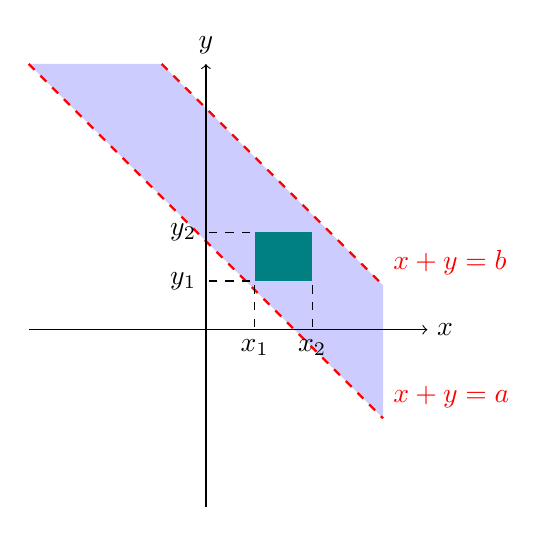
\begin{tikzpicture}[scale=0.75] % Scale everything to 3/4

        % Define parameters
        \def\a{1.5}  % Scaled to 3/4
        \def\b{3.75}  % Scaled to 3/4
        \def\xmin{-3}  % Scaled to 3/4
        \def\xmax{3}  % Scaled to 3/4
        \def\ymin{-3}  % Scaled to 3/4
        \def\ymax{3}  % Scaled to 3/4

        % Shade the region between the two lines
        \fill[blue!20] (\xmin, \a-\xmin) -- (\xmax, \a-\xmax) -- (\xmax, \b-\xmax) -- (-0.75, 4.5) -- cycle;

        % Draw the boundary lines
        \draw[thick, red, dashed] (\xmin, \a-\xmin) -- (\xmax, \a-\xmax) node[anchor=south west] {$x+y=a$};
        \draw[thick, red, dashed] (-0.75, 4.5) -- (\xmax, \b-\xmax) node[anchor=south west] {$x+y=b$};

        % Axes
        \draw[->] (\xmin, 0) -- (\xmax+0.75, 0) node[right] {$x$};
        \draw[->] (0, \ymin) -- (0, \ymax+1.5) node[above] {$y$};

        % square
        \fill[teal] (0.825, 0.825) rectangle (1.8, 1.65);

        % labels
        \draw[thin, black, dashed] (0.75, 0.825) -- (0, 0.825) node[left] {$y_1$};
        \draw[thin, black, dashed] (1.8, 0.75) -- (1.8, 0) node[below] {$x_2$};
        \draw[thin, black, dashed] (0.75, 1.65) -- (0, 1.65) node[left] {$y_2$};
        \draw[thin, black, dashed] (0.825, 0.75) -- (0.825, 0) node[below] {$x_1$};

    \end{tikzpicture}
\end{figure}
